% !TeX root = ../phd-thesis.tex

\begin{figure}
	\centering
	\begin{tabular}{c|c|c}
		Data set & Predictors & Extractors \\
		\hline\hline
		%\multirow{3}{*}{
		\subfloat[Sample distribution.]{
			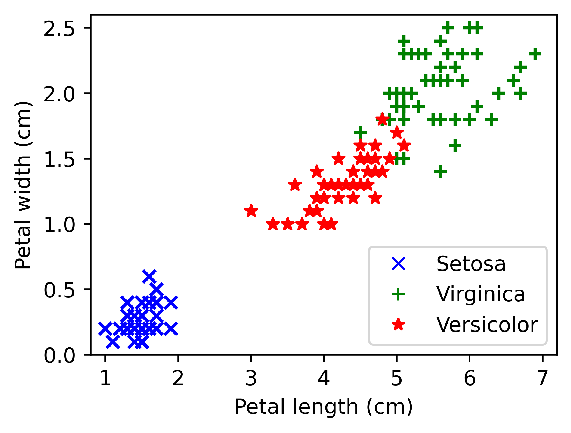
\includegraphics[width=0.21\linewidth]{figures/iris.pdf}
			\label{fig:iris}
			} %}
		&
		\subfloat[5-NN.]{
			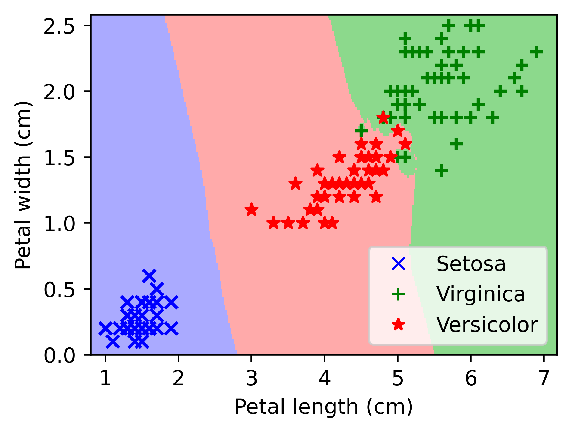
\includegraphics[width=0.21\linewidth]{figures/knn.pdf}
			\label{fig:knn}
		} &
		\subfloat[\real{}.]{
			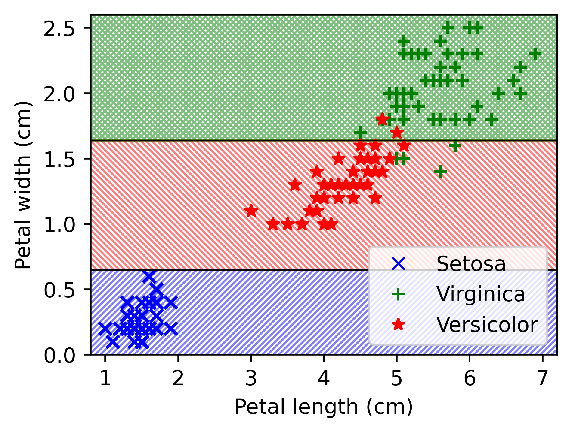
\includegraphics[width=0.21\linewidth]{figures/real.pdf}
			\label{fig:real}
		}
		\subfloat[\trepan{}.]{
			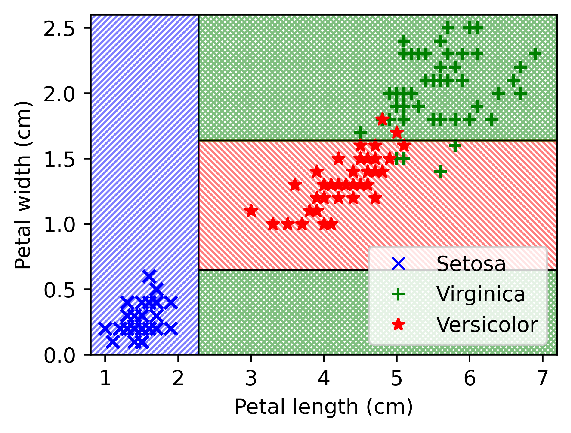
\includegraphics[width=0.21\linewidth]{figures/trepan.pdf}
			\label{fig:trepan}
		} \\
		&
		\subfloat[DT with cont. feat.]{
			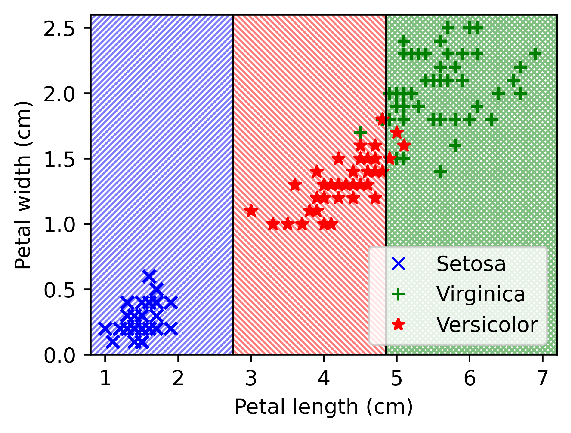
\includegraphics[width=0.21\linewidth]{figures/cartNoDisc.pdf}
			\label{fig:dt2}
		} &
		\subfloat[\cart{} with cont. feat.]{
			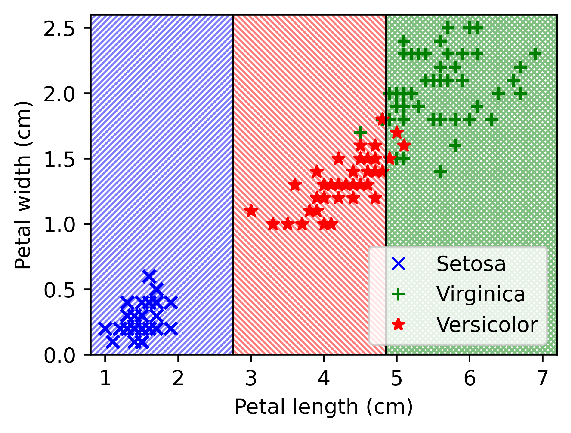
\includegraphics[width=0.21\linewidth]{figures/cartNoDisc.pdf}
			\label{fig:cart2}
		}\\
		&
		\subfloat[DT with binary feat.]{
			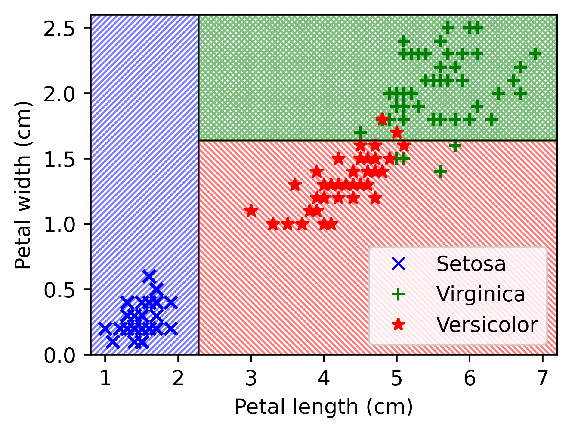
\includegraphics[width=0.21\linewidth]{figures/cart.pdf}
			\label{fig:dt}
		} &
		\subfloat[\cart{} with binary feat.]{
			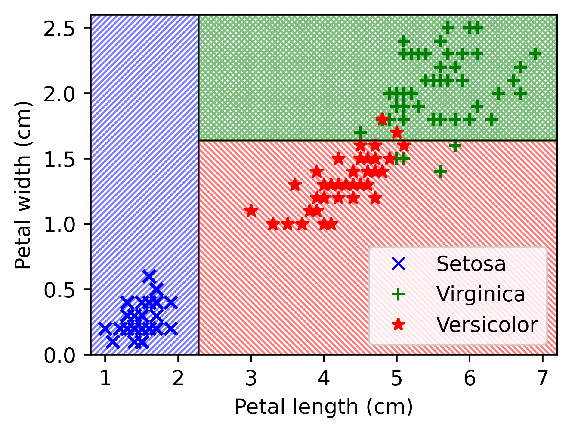
\includegraphics[width=0.21\linewidth]{figures/cart.pdf}
			\label{fig:cart}
		}\\
	\end{tabular}

	\caption{Comparison between Iris data set input space partitionings performed by the algorithms implemented in \psyke{}. Only the two most relevant features are reported---i.e., petal width and length.}
	\label{fig:irisAll}
\end{figure}